\chapter{Displeje}

    „\emph{V dnešní době jsou displeje a obrazovky naprosto neoddělitelnou součástí moderního života. Vždyť do nich koukáme po většinu každého dne!}~\cite{DisplejToply}“ Displej je zařízení, které zobrazuje informace (text, obrázky, znaky). Druhů displejů existuje opravdu spousta, například elektromechanické (překlápěcí, terčíkové, segmentové)~\cite{ElektromechanickeDispleje}, segmentové LED displeje a LED maticové displeje, LCD, OLED displeje, E-ink displeje a další. Základní parametry displejů jsou: úhlopříčka, rozlišení (počet pixelů, které dokáže zobrazit), obnovovací frekvence, odezva, jas a kontrast, barevná reprodukce a povrchová úprava~\cite{DisplejToply}.

    \section{Segmentové a maticové LED displeje}
        Segmentové displeje umožňují zobrazit číslice, znaky nebo symboly. Lze ovládat pouze jednotlivé segmenty, předurčené z výroby. Používají se v elektronických zařízeních, jako jsou měřící přístroje, hodiny, kalkulačky a další. Nejčastější typy jsou LCD segmentové displeje (viz obr.~\ref{LCDseg}) a LED segmentové displeje (viz obr.~\ref{LEDseg})~\cite{ZobrazovaciJednotky}.

        \begin{figure}[htb]
        \resizebox{8cm}{!}{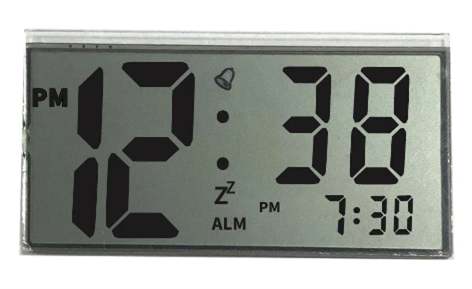
\includegraphics{LaTeX sablona IB/obrazky/LCD_seg_displej.png}}
        \caption{LCD segmentový displej~\cite{LCDsegDisplej}}
        \label{LCDseg}
        \end{figure}
        
        \begin{figure}[htb]
        \resizebox{8cm}{!}{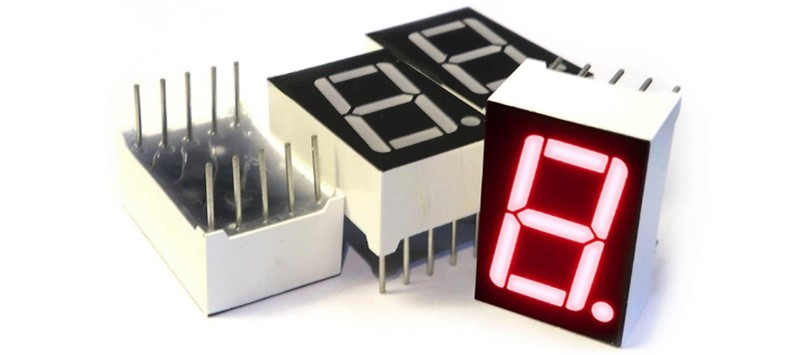
\includegraphics{LaTeX sablona IB/obrazky/LED_seg_displej.jpg}}
        \caption{LED 7 segmentový displej~\cite{7segmentdisplejPrincipAfunkcia}}
        \label{LEDseg}
        \end{figure}
        
        Maticové displeje se skládají z maticově uspořádaných LED. Používají se například jako informační tabule (viz obr.~\ref{LEDmat})~\cite{MaticovyLEDdisplej}.

        \begin{figure}[htb]
        \resizebox{8cm}{!}{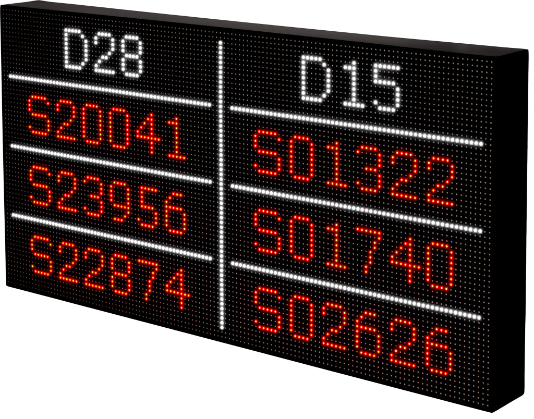
\includegraphics{LaTeX sablona IB/obrazky/maticovy_LED_displej.png}}
        \caption{maticový LED displej~\cite{MaticovyDisplej}}
        \label{LEDmat}
        \end{figure}

    \section{LCD}
        LCD (Liquid Crystal Display) funguje na principu tekutých krystalů, které jsou vloženy mezi dvě elektrody a polarizační filtry. Po připojení napájení na elektrody se uspořádání krystalů natáčí a tím mění své optické vlastnosti. U~barevných LCD se každý pixel dělí na 3 buňky - červenou, zelenou a modrou, přičemž u každé z nich lze díky natáčení krystalů zvlášť měnit jas.
        
        Využívají se jako obrazovky monitorů, televizí a různých přístrojů~\cite{DisplejeLCD}. Příklad takového displeje můžete vidět na obrázku~\ref{TFTLCD}. Na principu tekutých krystalů funguje také velká část segmentových displejů a znakových displejů s maticovými poli viz obr.~\ref{LCDalfn}. V dnešní době jsou větší obrazovky (ne ty segmentové) často nahrazovány OLED displeji - viz kapitola 2.3. Výhodou větších LCD obrazovek je, že jsou velmi ploché a mají poměrně nízkou spotřebu. Problémem těchto displejů je kontrast v tmavších barvách. Krystaly nedokáží zastavit všechno světlo, tudíž místo černé barvy zobrazí tmavý odstín šedé~\cite{ZobrazovaciGrafickaZarizeni}.

        \begin{figure}[htb]
        \resizebox{8cm}{!}{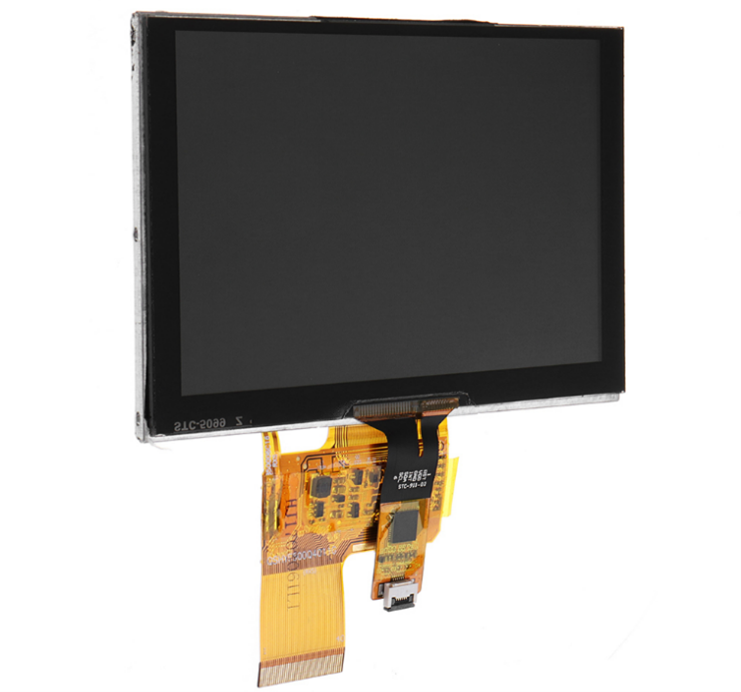
\includegraphics{LaTeX sablona IB/obrazky/LCD_TFT.png}}
        \caption{TFT LCD 800x480 dotykový~\cite{TFTLCDdisplej}}
        \label{TFTLCD}
        \end{figure}

        \begin{figure}[htb]
        \resizebox{8cm}{!}{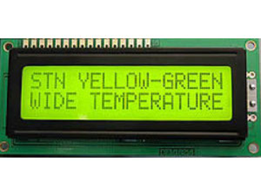
\includegraphics{LaTeX sablona IB/obrazky/LCD_alfn.png}}
        \caption{alfanumerický LCD~\cite{DisplejeLCD}}
        \label{LCDalfn}
        \end{figure}

    \clearpage

    \section{OLED displeje}
        OLED (Organic Light Emitting Diode) je jedna z nejnovějších zobrazovacích technologií. Využívá technologii organických elektroluminescenčních diod~\cite{ZobrazovaciGrafickaZarizeni}. Zde na rozdíl od LCD funguje každý pixel jako nezávislý zdroj světla. To umožňuje vyšší kontrast a úsporu energie. OLED displeje se používají v~mobilních telefonech, monitorech, televizích a v mnoha dalších přístrojích (obr.~\ref{OLED}). Nevýhodou těchto displejů je vypalování pixelů. Pokud bude pořád ve stejné části displeje dlouho svítit například nějaký znak, bude mírně vidět i po vypnutí obrazovky, nebo změně obrazu.

        \begin{figure}[htb]
        \resizebox{8cm}{!}{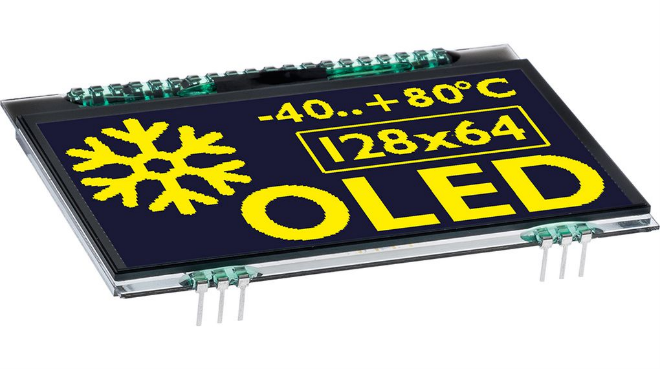
\includegraphics{LaTeX sablona IB/obrazky/oled.png}}
        \caption{OLED displej 128x64~\cite{OLEDDisplay}}
        \label{OLED}
        \end{figure}

    \section{E-ink displeje} \label{EinkKapitola}
        E-ink, E-paper, nebo také elektronický papír je technologie displeje, která se vzhledem velmi podobá klasickému papíru (obr.~\ref{EinkDisp}). Na rozdíl od většiny jiných způsobů zobrazování, kde jednotlivé pixely vyzařují světlo, zde pixely světlo pouze odráží (jako u obyčejného papíru s inkoustem). Tyto displeje jsou velmi úsporné, elektrickou energii potřebují jen při překreslení~\cite{EinkToply}. Takové překreslení ale většinou trvá kolem 1 až 3 sekund, proto nejsou vhodné pro aplikace, kde je potřeba rychlá obnovovací frekvence. Další nevýhodou je malá škála barev. Často mají k dispozici pouze pár odstínů šedé, avšak barevné displeje už také nejsou neobvyklé. Poměrně dlouhou dobu se používají v~elektronických čtečkách knih, nově také v supermarketech jako elektronické cenovky a začínají se objevovat v chytrých zařízeních jako jsou hodinky, mobilní telefony a monitory (viz obrázek~\ref{EinkMon}).

        \begin{figure}[htb]
        \resizebox{8cm}{!}{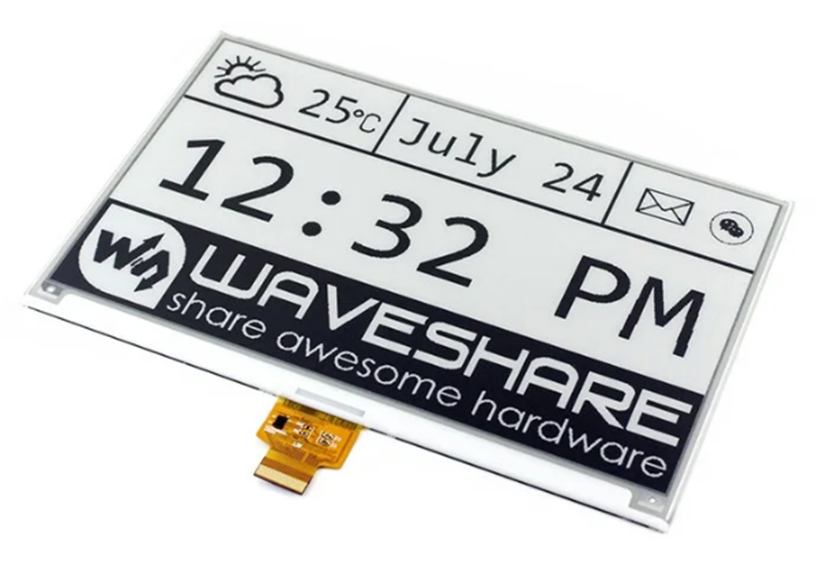
\includegraphics{LaTeX sablona IB/obrazky/eink_displej.png}}
        \caption{E-ink displej 7,5" 800x480px~\cite{E-Ink800x480px}}
        \label{EinkDisp}
        \end{figure}
        
        \begin{figure}[htb]
        \resizebox{8cm}{!}{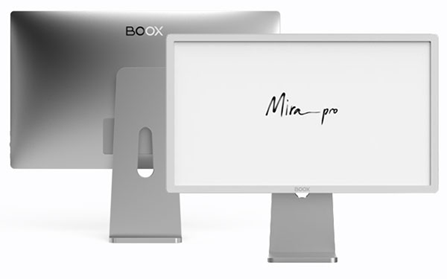
\includegraphics{LaTeX sablona IB/obrazky/eink_monitor.png}}
        \caption{E-ink monitor Onyx Boox Mira PRO, 25"~\cite{ONYXBOOXMIRAPRO}}
        \label{EinkMon}
        \end{figure}
